\documentclass[10pt]{article}
\usepackage{amsmath,amsfonts,times}
\usepackage{graphicx,color,tikz,pgfplots}
\usepackage[paperwidth=8cm,paperheight=9.0cm,lmargin=0in,rmargin=0in,tmargin=0.in,bmargin=0.in]{geometry}
\usepackage{bm}
\usetikzlibrary{arrows,shadings,shapes.arrows,decorations.pathreplacing,calc, positioning}
\usepgfplotslibrary{fillbetween}

\pgfplotsset{
  compat=newest,
  myStyle/.style={},
}

\newlength{\circleRadius}
\setlength{\circleRadius}{1.25pt}

\newlength{\cellWidth}
\setlength{\cellWidth}{3.2cm}

\newlength{\patchWidth}
\setlength{\patchWidth}{1cm}

\newlength{\partWidth}
\setlength{\partWidth}{1.25cm}

\def\N{15}
\def\seed{6}

\begin{document}
\centering
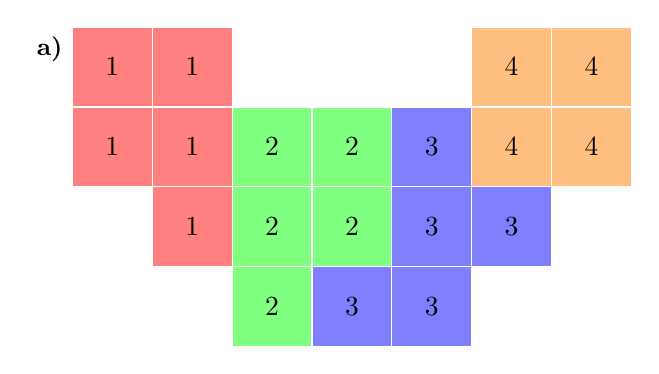
\begin{tikzpicture}[
    node distance=0\patchWidth,
    patch/.style={minimum width=\patchWidth, minimum height=\patchWidth, draw=none, inner sep=0 pt, rectangle},
    rank1/.style={patch, fill=red!50!white},
    rank2/.style={patch, fill=green!50!white},
    rank3/.style={patch, fill=blue!50!white},
    rank4/.style={patch, fill=orange!50!white},
  ]

  \node[rank1, alias=1] at (0,0)     {1};
  \node[rank1, alias=2,  right=of 1] {1};
  \node[rank1, alias=3,  below=of 1] {1};
  \node[rank1, alias=4,  right=of 3] {1};
  \node[rank2, alias=5,  right=of 4] {2};
  \node[rank2, alias=6,  right=of 5] {2};
  \node[rank3, alias=7,  right=of 6] {3};
  \node[rank4, alias=8,  right=of 7] {4};
  \node[rank4, alias=9,  right=of 8] {4};
  \node[rank4, alias=10, above=of 8] {4};
  \node[rank4, alias=11, above=of 9] {4};
  \node[rank1, alias=12, below=of 4] {1};
  \node[rank2, alias=13, right=of 12] {2};
  \node[rank2, alias=14, right=of 13] {2};
  \node[rank3, alias=15, right=of 14] {3};
  \node[rank3, alias=16, right=of 15] {3};
  \node[rank2, alias=17, below=of 13] {2};
  \node[rank3, alias=18, below=of 14] {3};
  \node[rank3, alias=19, below=of 15] {3};

  \node[font=\small, anchor=north east, below left=of 1.north west] {\bfseries a)};
\end{tikzpicture}
\vfill
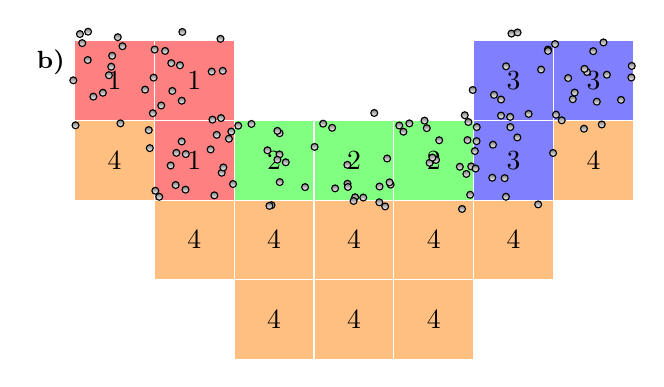
\begin{tikzpicture}[
    node distance=0\patchWidth,
    patch/.style={minimum width=\patchWidth, minimum height=\patchWidth, draw=none, inner sep=0 pt, rectangle},
    rank1/.style={patch, fill=red!50!white},
    rank2/.style={patch, fill=green!50!white},
    rank3/.style={patch, fill=blue!50!white},
    rank4/.style={patch, fill=orange!50!white},
  ]

  \node[rank1, alias=1] at (0,0)     {1};
  \node[rank1, alias=2,  right=of 1] {1};
  \node[rank4, alias=3,  below=of 1] {4};
  \node[rank1, alias=4,  right=of 3] {1};
  \node[rank2, alias=5,  right=of 4] {2};
  \node[rank2, alias=6,  right=of 5] {2};
  \node[rank2, alias=7,  right=of 6] {2};
  \node[rank3, alias=8,  right=of 7] {3};
  \node[rank4, alias=9,  right=of 8] {4};
  \node[rank3, alias=10, above=of 8] {3};
  \node[rank3, alias=11, above=of 9] {3};
  \node[rank4, alias=12, below=of 4] {4};
  \node[rank4, alias=13, right=of 12] {4};
  \node[rank4, alias=14, right=of 13] {4};
  \node[rank4, alias=15, right=of 14] {4};
  \node[rank4, alias=16, right=of 15] {4};
  \node[rank4, alias=17, below=of 13] {4};
  \node[rank4, alias=18, below=of 14] {4};
  \node[rank4, alias=19, below=of 15] {4};

  
  \foreach \i in {1,...,\N}{
    \shade[fill=black!50!white, draw=black] (1)  + (rnd*\partWidth - 0.5*\partWidth, rnd*\partWidth - 0.5*\partWidth) circle(\circleRadius);
    \shade[fill=black!50!white, draw=black] (2)  + (rnd*\partWidth - 0.5*\partWidth, rnd*\partWidth - 0.5*\partWidth) circle(\circleRadius);
    \shade[fill=black!50!white, draw=black] (4)  + (rnd*\partWidth - 0.5*\partWidth, rnd*\partWidth - 0.5*\partWidth) circle(\circleRadius);
    \shade[fill=black!50!white, draw=black] (5)  + (rnd*\partWidth - 0.5*\partWidth, rnd*\partWidth - 0.5*\partWidth) circle(\circleRadius);
    \shade[fill=black!50!white, draw=black] (6)  + (rnd*\partWidth - 0.5*\partWidth, rnd*\partWidth - 0.5*\partWidth) circle(\circleRadius);
    \shade[fill=black!50!white, draw=black] (7)  + (rnd*\partWidth - 0.5*\partWidth, rnd*\partWidth - 0.5*\partWidth) circle(\circleRadius);
    \shade[fill=black!50!white, draw=black] (8)  + (rnd*\partWidth - 0.5*\partWidth, rnd*\partWidth - 0.5*\partWidth) circle(\circleRadius);
    \shade[fill=black!50!white, draw=black] (10) + (rnd*\partWidth - 0.5*\partWidth, rnd*\partWidth - 0.5*\partWidth) circle(\circleRadius);
    \shade[fill=black!50!white, draw=black] (11) + (rnd*\partWidth - 0.5*\partWidth, rnd*\partWidth - 0.5*\partWidth) circle(\circleRadius);
  }

  \node[font=\small, anchor=north east, below left=of 1.north west] {\bfseries b)};
\end{tikzpicture}

\end{document} 
